%!TEX root=paper/paper.tex
\subsection{MDP Formulation}\label{sec:mdp_formulation}

To model the \textbf{action selection} policy $\pi(x): \mathcal{X} \mapsto 2^\mathcal{A}$, we introduce the Markov Decision Process (MDP), which defines a single \emph{episode} of selecting actions for some instance $x$.

\begin{mydef} \label{def:MDP}
The \textbf{feature selection MDP} consists of the tuple $(\mathcal{S}, \mathcal{A}, T(\cdot), R(\cdot), \gamma)$:

\begin{itemize}
\item \textbf{State} $s \in \mathcal{S}$ stores the selected action subset $\mathcal{A}_{\pi(x)}$, resulting observations, and total cost $C_{\mathcal{A}_{\pi(x)}}$.
\item The set of \textbf{actions} $\mathcal{A}$.
\item The \textbf{state transition} distribution $T(s' \mid s, a)$ can depend on the instance $x$.
\item The \textbf{reward} function $R(s, a, s') \mapsto \mathbb{R}$ is manually specified, and depends on the actions taken and the instance $x$.
\item The discount $\gamma$ determines amount of \textbf{lookahead} in selecting actions: if 0, actions are selected greedily based on their immediate reward; if 1, the reward accrued by subsequent actions is given just as much weight as the reward of the current action.
\end{itemize}
\end{mydef}

\PM{Trajectories and reward}
A recognition \emph{episode} takes an image $\mathcal{I}$ and proceeds from the initial state $s^0$ and action $a^0$ to the next pair $(s^1,a^1)$, and so on until $(s^J,a^J)$, where $J$ is the last step of the process with $t \le T_d$.
At that point, the policy is terminated, and a new episode can begin on a new image.
We call this a \emph{trajectory} $\xi = (s_0, a_0, s_1, r_1, \dots, a_{I-1}, s_I, r_I)$, where $I$ is the total number of actions taken (and therefore features selected), $s_0$ is the initial state, $a_i \sim \pi(a \mid s_i)$ is chosen by the \emph{policy} $\pi(a \mid s)$, and $s_{i+1} \sim T(s \mid s_i, a_i)$, which can depend on $x$.
The total expected reward (value) of an MDP episode is written as
\begin{equation}\label{eq:expected_reward}
V_\pi(s_0) =
\mathbb{E}_{\xi \sim \left\{ \pi, x \right\}} r(\xi) =
\mathbb{E}_{\xi \sim \left\{ \pi, x \right\}} \left[ \sum_{i=0}^I \gamma^i \, r_i \right]
\end{equation}

\PM{Q-Value function}
We seek $\pi$ that maximizes \autoref{eq:expected_reward}.
If we had a function accurately predicting the value of taking an action in a state, we could define the policy as simply taking the action with maximum value from any state.
We specify this function $Q(s,a): S \times \mathcal{A} \mapsto \mathbb{R}$, where $S$ is the space of all possible states, to assign a value to a potential action $a \in \mathcal{A}$ given the current state $s$ of the decision process.
We can then define the policy $\pi$ as simply $\argmax_{a_i \in \mathcal{A} \setminus \mathcal{O}} Q(s,a_i)$.
The Q-function is defined and learned recursively:
\begin{align}\label{eq:recursive_value}
Q^\pi(s^j,a) = \mathbb{E}_{s^{j+1}} [R(s^j,a) + \gamma Q^\pi(s^{j+1},\pi(s^{j+1}))]
\end{align}

\subsection{Learning the policy}
\PM{Function approximation}
Although the action space $\mathcal{A}$ is manageable, the space of possible states $S$ is intractable, and we must use function approximation to represent $Q(s,a)$: a common technique in reinforcement learning \parencite{Sutton1998}.
We featurize the state-action pair and assume linear structure:
\begin{align}\label{eq:policy}
Q^\pi(s,a) = \theta_\pi^\top \phi(s,a)
\end{align}
where $\phi: \mathcal{S} \times \mathcal{A} \mapsto \mathbb{R}^{d_s}$ is the state featurization function, $d_s$ is the dimensionality of the state feature vector, and $\theta^\pi$ is a vector of weights that defines the policy $\pi$.

\PM{Policy function}
Specifically, the policy is defined as
\begin{equation}
\pi(a \mid s) = \frac{1}{Z} \exp\left(\frac{1}{\tau} \theta^T \phi(s, a)\right)
\end{equation}
where $Z$ is the appropriate normalization and $\tau$ is a temperature parameter that controls the level of exploration vs. exploitation in the policy.
As $\tau \rightarrow 0$, ${\pi(a \mid s)}$ becomes highly peaked at $\argmax_a Q(s,a)$; it becomes uniform as $\tau \rightarrow \infty$.
In training, this parameter is turned down gradually.

\begin{figure}[ht]
\centering
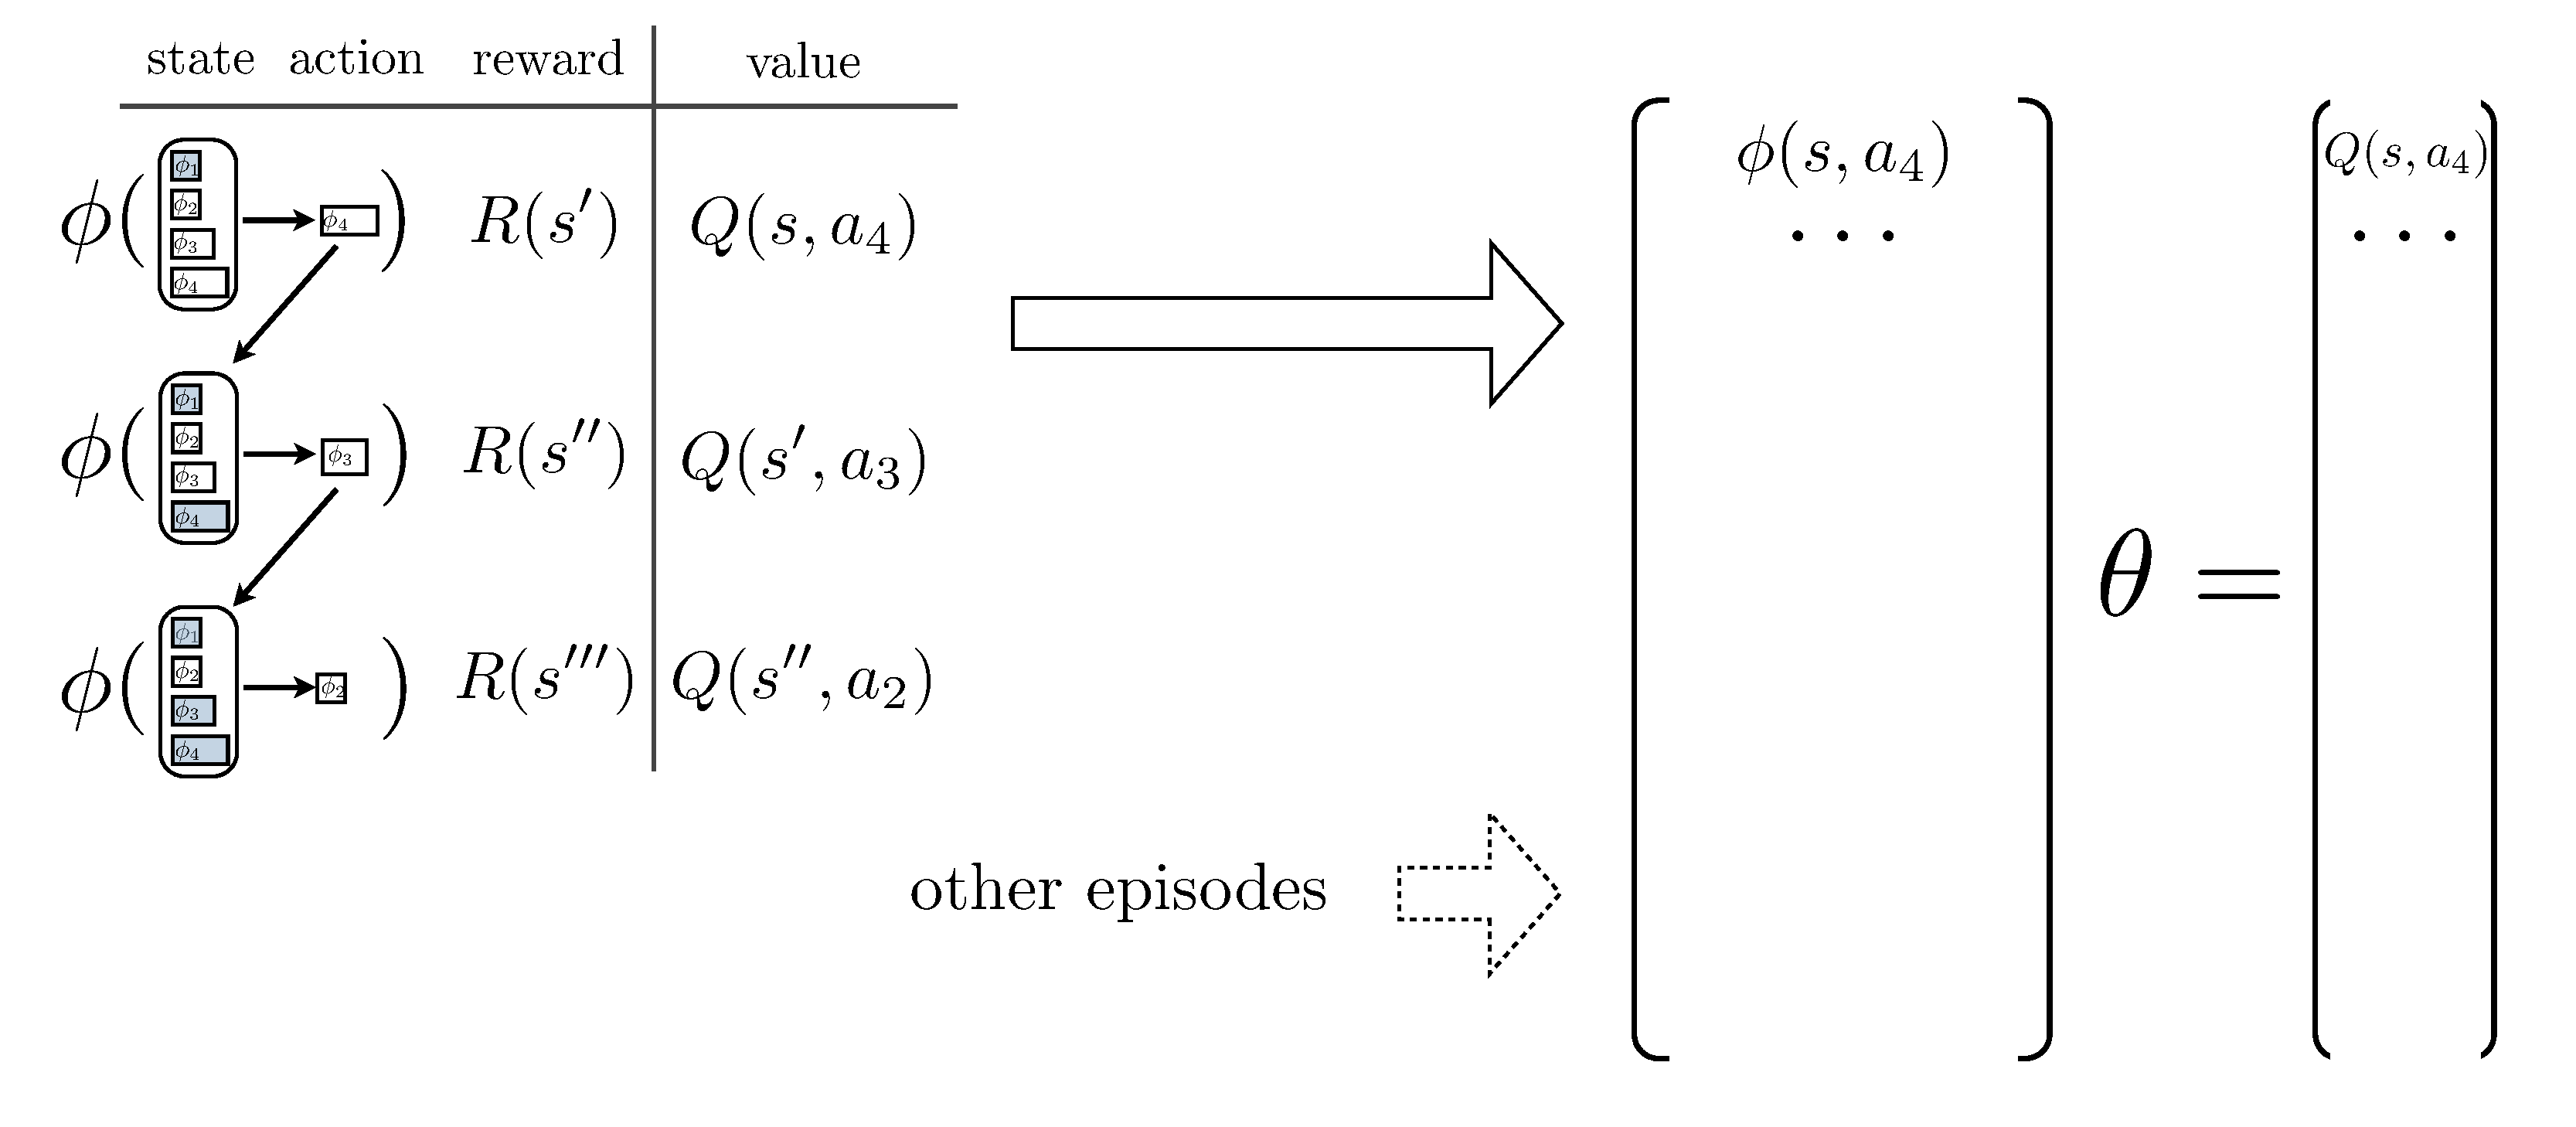
\includegraphics[width=\linewidth]{../../figures/qiteration_explanation.pdf}
\caption[
Explanation of the Q-iteration method.]{
We sample $Q^\pi(s, a) = \mathbb{E}_{s'} \left[ R(s') + \gamma Q^\pi(s', \pi(s')) \right] = \theta^T \phi(s, a)$ by running the policy over many images.
Once an episode is complete, the $Q$-value at each $(s, a)$ can be determined.
To update the policy, simply minimize the prediction error of $\theta$, and repeat.
\label{fig:qiteration_explanation}}
\end{figure}


\PM{Sampling Q-function}
While we can't directly compute the expectation in \autoref{eq:recursive_value}, we can sample it by running actual episodes to gather $<s,a,r,s'>$ samples, where $r$ is the reward obtained by taking action $a$ in state $s$, and $s'$ is the following state.
We then learn the optimal policy by repeatedly gathering samples with the current policy, minimizing the error between the discounted reward to the end of the episode as predicted by our current $Q(s^j,a)$ and the actual values gathered, and updating the policy with the resulting weights.
This method is akin to fitted Q-iteration, a variant of generalized policy iteration \parencite{Ernst2005,Sutton1998}.
\autoref{fig:qiteration_explanation} shows a step of this process.

\PM{Gathering trajectories}
During training, we gather samples starting from either a random feasible state, with probability $\epsilon$, or from the initial empty state otherwise.
Both $\epsilon$ and $\tau$ parameters decay exponentially with the number of training iterations.
Training is terminated if $\pi_{\theta_{i+1}}$ returns the exact same sequence of episodes $\xi$ on a validation set as $\pi_{\theta_{i}}$.
During test time, $\epsilon$ is set to $0.05$.

\PM{Block-coding}
To formulate learning the policy as a single regression problem, we could represent the features in block form, where $\phi(s,a)$ is a vector of size $F|\mathcal{A}|$, with all values set to $0$ except for the $F$-sized block corresponding to $a$.
An implementation detail: instead of block-coding $\phi(s,a)$, we learn $F$ separate $\theta_f$'s for the features $\phi(s)$: one for each action $a$
To prevent overfitting, we use $L_2$-regularized regression.
The weight $\alpha$ of the regularization term is tied across the $F$ separate regressions and is tuned by cross-validation on 3 folds.

\PM{Details}
We run $15$ iterations of accumulating samples by running $350$ episodes, starting with a baseline policy which will be described in \autoref{sec:det_evaluation}, and cross-validating the regularization parameter at each iteration.
Samples are not thrown away between iterations.

\subsubsection{Greedy vs non-myopic}

\PM{Greedy}
Note from \autoref{eq:recursive_value} that the $\gamma \in [0,1]$ parameter of the MDP controls the level of \emph{discounting} of rewards of future action in computing the value \autoref{eq:expected_reward}.
In the baseline \textbf{greedy} setting, with $\gamma=0$, rewards gained by future actions are not counted at all in determining the value of the current action.
The value function is determined entirely by the immediate reward, and so only completely greedy policies can be learned in this case.
This setting is used as baseline.

\PM{Non-myopic}
In the \textbf{non-myopic} setting, with $\gamma=1$, rewards gained by future actions are valued exactly as much as reward gained by the current action in determining its value.
However, a slightly lower value of $\gamma$ mitigates the effects of increasing uncertainty regarding the state transitions over long episodes.
We set this meta-parameter of our approach through cross-validation, and find that a mid-level value ($0.4$) works best.
